% UAI 2026 Poster - Reorganized design version
% Author: Chorok Lee, KAIST
% A0 Portrait: 84.1cm x 118.9cm

\documentclass[a4paper]{article}
\usepackage[paperwidth=84.1cm,paperheight=118.9cm,margin=1.5cm]{geometry}
\usepackage[utf8]{inputenc}
\usepackage[T1]{fontenc}
\usepackage{lmodern}
\usepackage{amsmath,amssymb}
\usepackage{graphicx}
\usepackage{booktabs}
\usepackage{tikz}
\usetikzlibrary{shapes,arrows.meta,positioning,calc,shadows}
\usepackage{xcolor}
\usepackage{colortbl}
\usepackage{array}
\usepackage{helvet}
\renewcommand{\familydefault}{\sfdefault}
\pagestyle{empty}
\setlength{\emergencystretch}{1.5em}

\definecolor{uaiblue}{RGB}{0,82,147}
\definecolor{uaiorange}{RGB}{232,119,34}
\definecolor{uailight}{RGB}{240,248,255}
\definecolor{uaidark}{RGB}{30,30,30}
\definecolor{alertred}{RGB}{200,50,50}
\definecolor{successgreen}{RGB}{46,139,87}
\definecolor{goldaccent}{RGB}{255,193,7}

\newcommand{\pct}{\char37}

\newcommand{\posterbox}[2]{%
\begin{tikzpicture}
\node[draw=uaiblue, line width=2.2pt, fill=white, rounded corners=8pt, inner sep=16pt, text width=0.93\linewidth, align=left, drop shadow={shadow xshift=1.4pt, shadow yshift=-1.4pt, opacity=0.10}] (box) {#2};
\node[fill=uaiblue, text=white, font=\bfseries\LARGE, rounded corners=4pt, inner sep=9pt, anchor=south west] at ($(box.north west)+(0.45cm,-0.22cm)$) {#1};
\end{tikzpicture}
}

\newcommand{\alertbox}[2]{%
\begin{tikzpicture}
\node[draw=uaiorange, line width=2.6pt, fill=white, rounded corners=8pt, inner sep=16pt, text width=0.93\linewidth, align=left, drop shadow={shadow xshift=1.4pt, shadow yshift=-1.4pt, opacity=0.10}] (box) {#2};
\node[fill=uaiorange, text=white, font=\bfseries\LARGE, rounded corners=4pt, inner sep=9pt, anchor=south west] at ($(box.north west)+(0.45cm,-0.22cm)$) {#1};
\end{tikzpicture}
}

\newcommand{\herobox}[2]{%
\begin{tikzpicture}
\node[draw=uaiorange, line width=3.2pt, fill=uailight, rounded corners=9pt, inner sep=18pt, text width=0.94\linewidth, align=left, drop shadow={shadow xshift=1.8pt, shadow yshift=-1.8pt, opacity=0.13}] (box) {#2};
\node[fill=uaiorange, text=white, font=\bfseries\huge, rounded corners=5pt, inner sep=11pt, anchor=south west] at ($(box.north west)+(0.45cm,-0.28cm)$) {#1};
\end{tikzpicture}
}

\newcommand{\bottomcard}[2]{%
\begin{minipage}[t]{0.31\linewidth}
{\fontsize{24}{29}\selectfont\bfseries\color{uaiblue}#1}\par\vspace{0.35em}
{\fontsize{19}{24}\selectfont #2}
\end{minipage}}

\begin{document}

%==============================================================================
% TITLE
%==============================================================================
\begin{center}

\begin{tikzpicture}
\node[fill=uaiblue!8, rounded corners=14pt, inner sep=0pt, drop shadow={shadow xshift=2pt, shadow yshift=-2pt, opacity=0.10}] {
\begin{minipage}{0.98\textwidth}
\vspace{0.75cm}
\centering
{\fontsize{72}{86}\selectfont\bfseries\color{uaiblue}Diagnosing Conformal Prediction Failures Under Distribution Shift}\\[0.55cm]
{\fontsize{44}{52}\selectfont\color{uaidark}A COVID-19 Case Study}\\[0.85cm]
{\fontsize{38}{46}\selectfont\color{uaidark}\textbf{Chorok Lee} \quad $\cdot$ \quad KAIST}\\[0.45cm]
{\fontsize{30}{36}\selectfont\color{uaiorange}\textbf{UAI 2026 --- Amsterdam, Netherlands}}
\vspace{0.55cm}
\end{minipage}
};
\end{tikzpicture}
\end{center}

\vspace{0.55cm}

%==============================================================================
% SUMMARY BANNER
%==============================================================================
\begin{center}
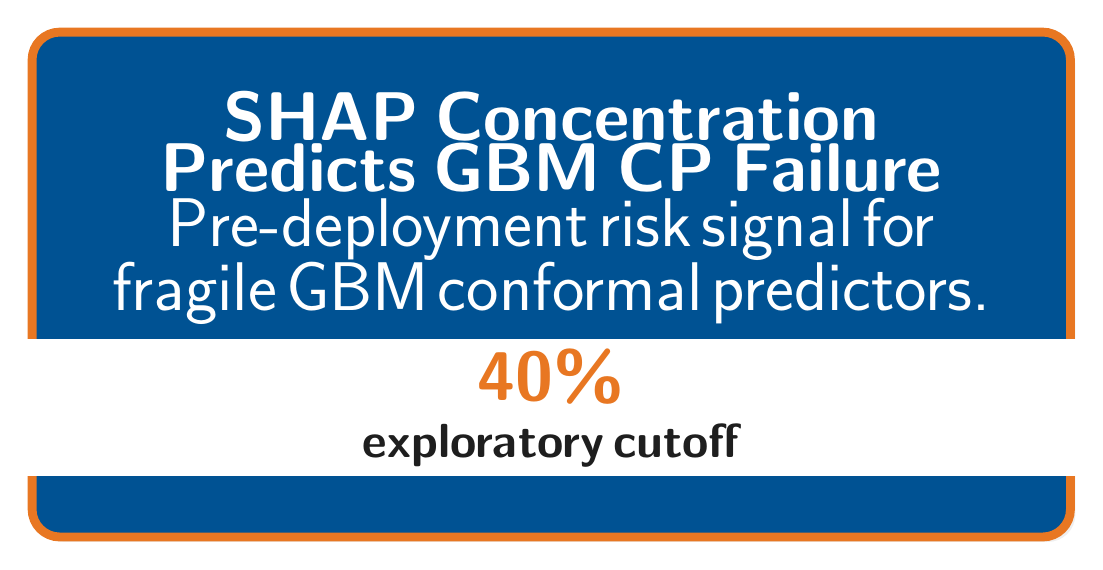
\begin{tikzpicture}
\node[fill=uaiblue, draw=uaiorange, line width=3.2pt, rounded corners=10pt, inner sep=22pt, text width=0.96\textwidth, drop shadow={shadow xshift=1.8pt, shadow yshift=-1.8pt, opacity=0.13}] {
\centering
{\fontsize{38}{45}\selectfont\color{white}\bfseries SHAP\hspace{0.22em}Concentration\hspace{0.22em}Predicts\hspace{0.22em}GBM\hspace{0.22em}CP\hspace{0.22em}Failure}\\[0.16em]
{\fontsize{24}{30}\selectfont\color{white}Pre-deployment risk signal for fragile GBM conformal predictors.}\\[0.46em]
\makebox[\linewidth][c]{%
\begin{tabular}{@{}c@{\hspace{1.2cm}}c@{\hspace{1.2cm}}c@{}}
\fcolorbox{white}{white}{\parbox{15.0cm}{\centering\fontsize{30}{36}\selectfont\color{uaiblue}\bfseries\boldmath $\rho = 0.853$\\[-0.05em]\fontsize{18}{22}\selectfont\color{uaidark}primary correlation, $n=16$}} &
\fcolorbox{white}{white}{\parbox{15.0cm}{\centering\fontsize{30}{36}\selectfont\color{uaiorange}\bfseries 40\pct\\[-0.05em]\fontsize{18}{22}\selectfont\color{uaidark}exploratory cutoff}} &
\fcolorbox{white}{white}{\parbox{15.0cm}{\centering\fontsize{30}{36}\selectfont\color{successgreen}\bfseries 91.7\pct\\[-0.05em]\fontsize{18}{22}\selectfont\color{uaidark}SALT+WILDS check}}
\end{tabular}}
};
\end{tikzpicture}
\end{center}

\vspace{0.6cm}

%==============================================================================
% THREE-COLUMN BODY
%==============================================================================
\begin{minipage}[t]{0.29\textwidth}
\vspace{0pt}

\posterbox{Problem \& Study Setting}{%
\vspace{0.85cm}
\fontsize{26}{32}\selectfont
\raggedright
\textbf{Conformal Prediction (CP)} gives uncertainty sets with coverage guarantees. Under deployment shift, those guarantees can break.

\vspace{0.65em}
\textbf{\color{uaiblue}Research Question:}
\begin{center}
\fcolorbox{uaiblue}{uailight}{\parbox{0.88\linewidth}{\centering\fontsize{24}{30}\selectfont
Can we \textbf{predict} when CP fails \textbf{before} deployment?
}}
\end{center}

\vspace{0.65em}
\begin{center}
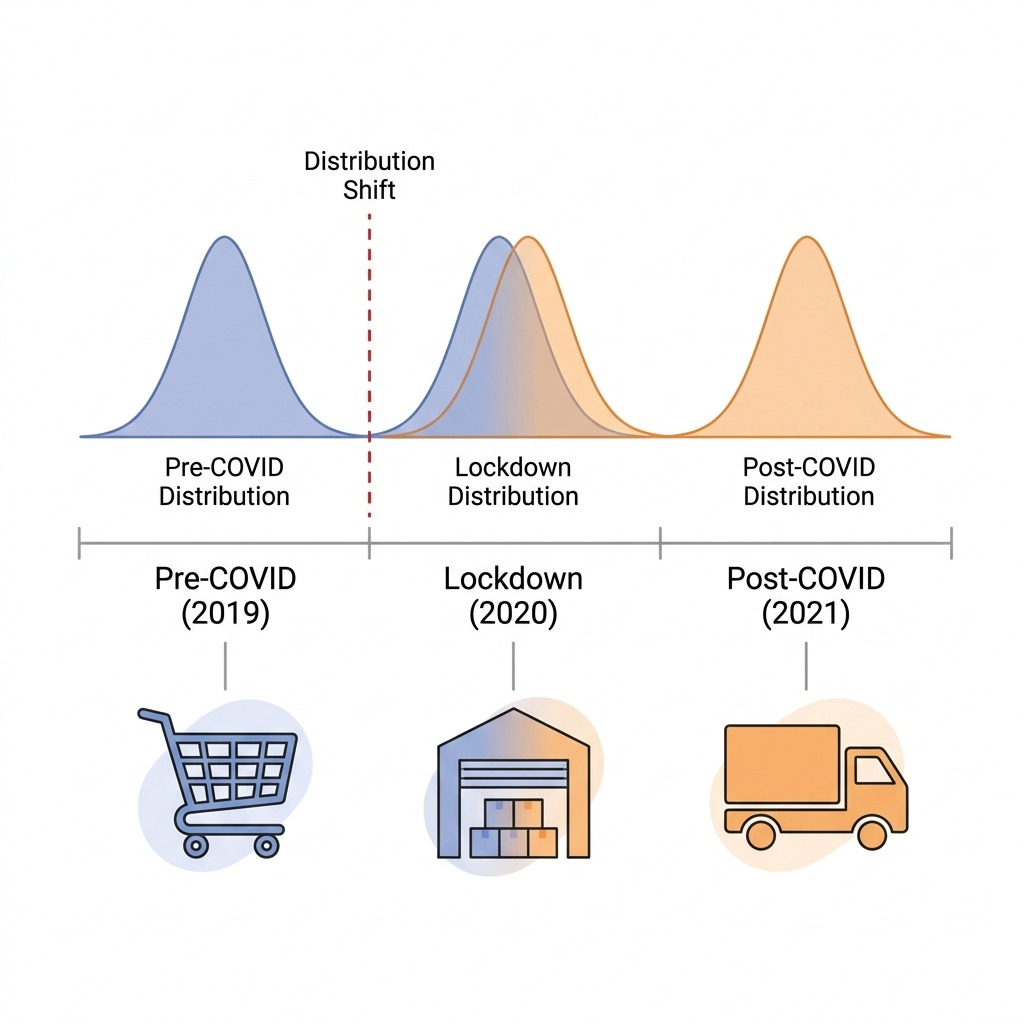
\includegraphics[width=0.92\linewidth]{../figures/fig1_covid_timeline.jpg}
\end{center}
{\fontsize{19}{23}\selectfont\textit{Fig 1: CP is calibrated pre-COVID, then tested after behavior changes.}}

\vspace{0.6em}
\fcolorbox{uaiblue}{white}{\parbox{0.92\linewidth}{%
{\fontsize{21}{26}\selectfont
\textbf{Analysis set}\par
SALT COVID shift: \textbf{8 tasks}\par
External multiclass endpoint: \textbf{+8 tasks}\par
Primary correlation: \textbf{$n=16$ across 9 domains}
}
}}
}

\vspace{0.75cm}

\posterbox{Diagnostic \& Theorem}{%
\vspace{0.75cm}
\fontsize{25}{31}\selectfont
\textbf{SHAP Concentration}
\begin{center}
\fcolorbox{uaiblue}{uailight}{\parbox{0.9\linewidth}{\centering
\vspace{0.25em}
{\fontsize{32}{39}\selectfont $\displaystyle C = \frac{\phi_1}{\sum_{j=1}^{p}\phi_j}$}\\[-0.02em]
{\fontsize{17}{21}\selectfont $\phi_j$: mean absolute SHAP importance; $\phi_1$: top-ranked feature}
\vspace{0.25em}
}}
\end{center}

\vspace{0.45em}
\fcolorbox{uaiblue}{white}{\parbox{0.92\linewidth}{\centering
\vspace{0.25em}
{\fontsize{19}{24}\selectfont\bfseries\color{uaiblue}Theorem (idealized additive model): concentration worsens APS score and coverage bounds}\\[0.05em]
{\fontsize{18}{22}\selectfont $\displaystyle \mathbb{E}[s_{\mathrm{test}}] \geq C(1-(K-1)\epsilon)+(1-C)(1-(K-1)\bar h)$}\\[0.15em]
{\fontsize{17}{21}\selectfont If $\epsilon < \bar h$, the score bound increases with $C$; the coverage upper bound is non-increasing in $C$.}
\vspace{0.25em}
}}

\vspace{0.65em}
\begin{center}
\begin{tabular}{ccc}
\fcolorbox{successgreen}{green!10}{\parbox{3.25cm}{\centering\vspace{0.15em}\color{successgreen}\fontsize{26}{32}\selectfont\bfseries $<$35\pct\\[-0.02em]\fontsize{18}{22}\selectfont\color{uaidark}Lower risk\vspace{0.15em}}} &
\fcolorbox{uaiorange}{goldaccent!18}{\parbox{3.25cm}{\centering\vspace{0.15em}\color{uaiorange}\fontsize{24}{30}\selectfont\bfseries\mbox{35--45\pct}\\[-0.02em]\fontsize{18}{22}\selectfont\color{uaidark}Monitor\vspace{0.15em}}} &
\fcolorbox{alertred}{red!10}{\parbox{3.25cm}{\centering\vspace{0.15em}\color{alertred}\fontsize{26}{32}\selectfont\bfseries $>$45\pct\\[-0.02em]\fontsize{18}{22}\selectfont\color{uaidark}Check factors\vspace{0.15em}}}
\end{tabular}
\end{center}
}

\end{minipage}%
\hfill
\begin{minipage}[t]{0.40\textwidth}
\vspace{0pt}

\herobox{MAIN RESULT}{%
\vspace{0.75cm}
\begin{center}
{\fontsize{34}{41}\selectfont\bfseries\color{uaidark}SHAP\hspace{0.18em}Concentration\hspace{0.18em}Predicts\hspace{0.18em}Coverage\hspace{0.18em}Drop}\\[-0.05em]
{\fontsize{23}{28}\selectfont\color{uaidark}Primary endpoint: 16 multiclass tasks across 9 domains}
\end{center}

\vspace{0.25em}
\begin{center}
\fcolorbox{uaiorange}{goldaccent!15}{\parbox{0.74\linewidth}{\centering
{\fontsize{19}{23}\selectfont\bfseries\color{uaidark}Scope: GBM multiclass classifiers, $K\geq4$}
}}
\end{center}

\vspace{0.45em}
\begin{center}
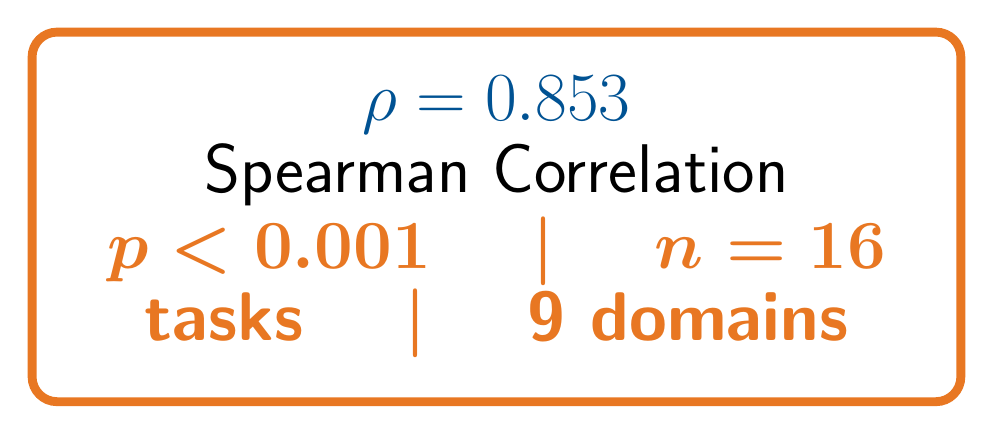
\begin{tikzpicture}
\node[fill=white, draw=uaiorange, line width=3.2pt, rounded corners=9pt, inner sep=16pt] {
\begin{minipage}{0.88\linewidth}
\centering
{\fontsize{116}{134}\selectfont\bfseries\color{uaiblue} $\rho = 0.853$}\\[0.28em]
{\fontsize{32}{40}\selectfont Spearman Correlation}\\[0.3em]
{\fontsize{28}{34}\selectfont\bfseries\boldmath\color{uaiorange} $p < 0.001$ \quad $\vert$ \quad $n = 16$ tasks \quad $\vert$ \quad 9 domains}
\end{minipage}
};
\end{tikzpicture}
\end{center}

\vspace{0.75em}
\begin{center}
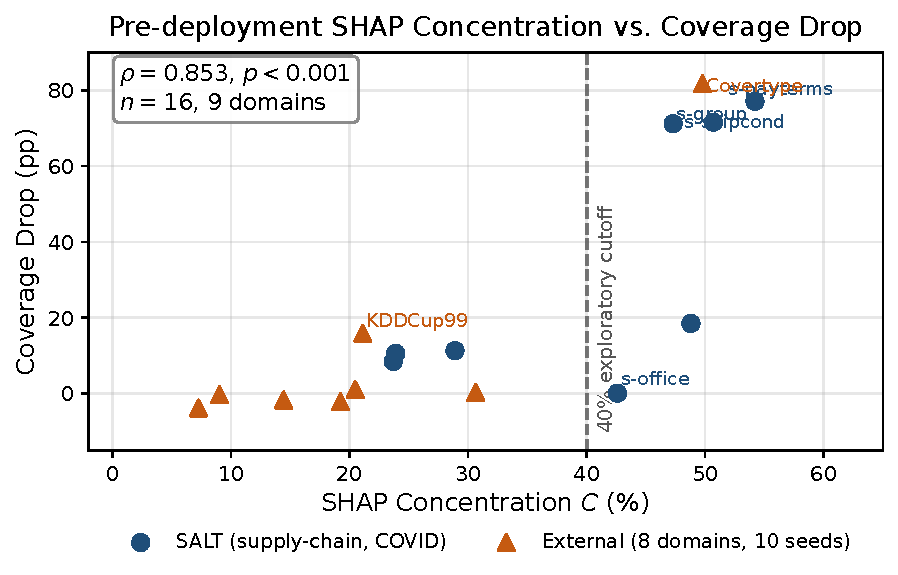
\includegraphics[width=0.92\linewidth]{../figures/figure_n16_correlation.pdf}
\end{center}
{\fontsize{18}{21}\selectfont\itshape Fig 3: Each point is a task; x-axis = pre-deployment SHAP concentration, y-axis = post-shift coverage drop.\par}
\vspace{0.15em}
\begin{center}
\fcolorbox{uaiblue}{uailight}{\parbox{0.94\linewidth}{\centering
\vspace{0.18em}
{\fontsize{23}{28}\selectfont\bfseries\color{uaiblue}Takeaway: higher concentration tracks larger CP coverage loss.}\\[-0.02em]
{\fontsize{17}{20}\selectfont Across 16 tasks, high-$C$ models occupy the high-drop region.}
\vspace{0.18em}
}}
\end{center}
}

\vspace{0.75cm}

\posterbox{Mechanism: Concentrated Dependence}{%
\vspace{0.75cm}
\fontsize{25}{31}\selectfont
\begin{center}
\makebox[\linewidth][c]{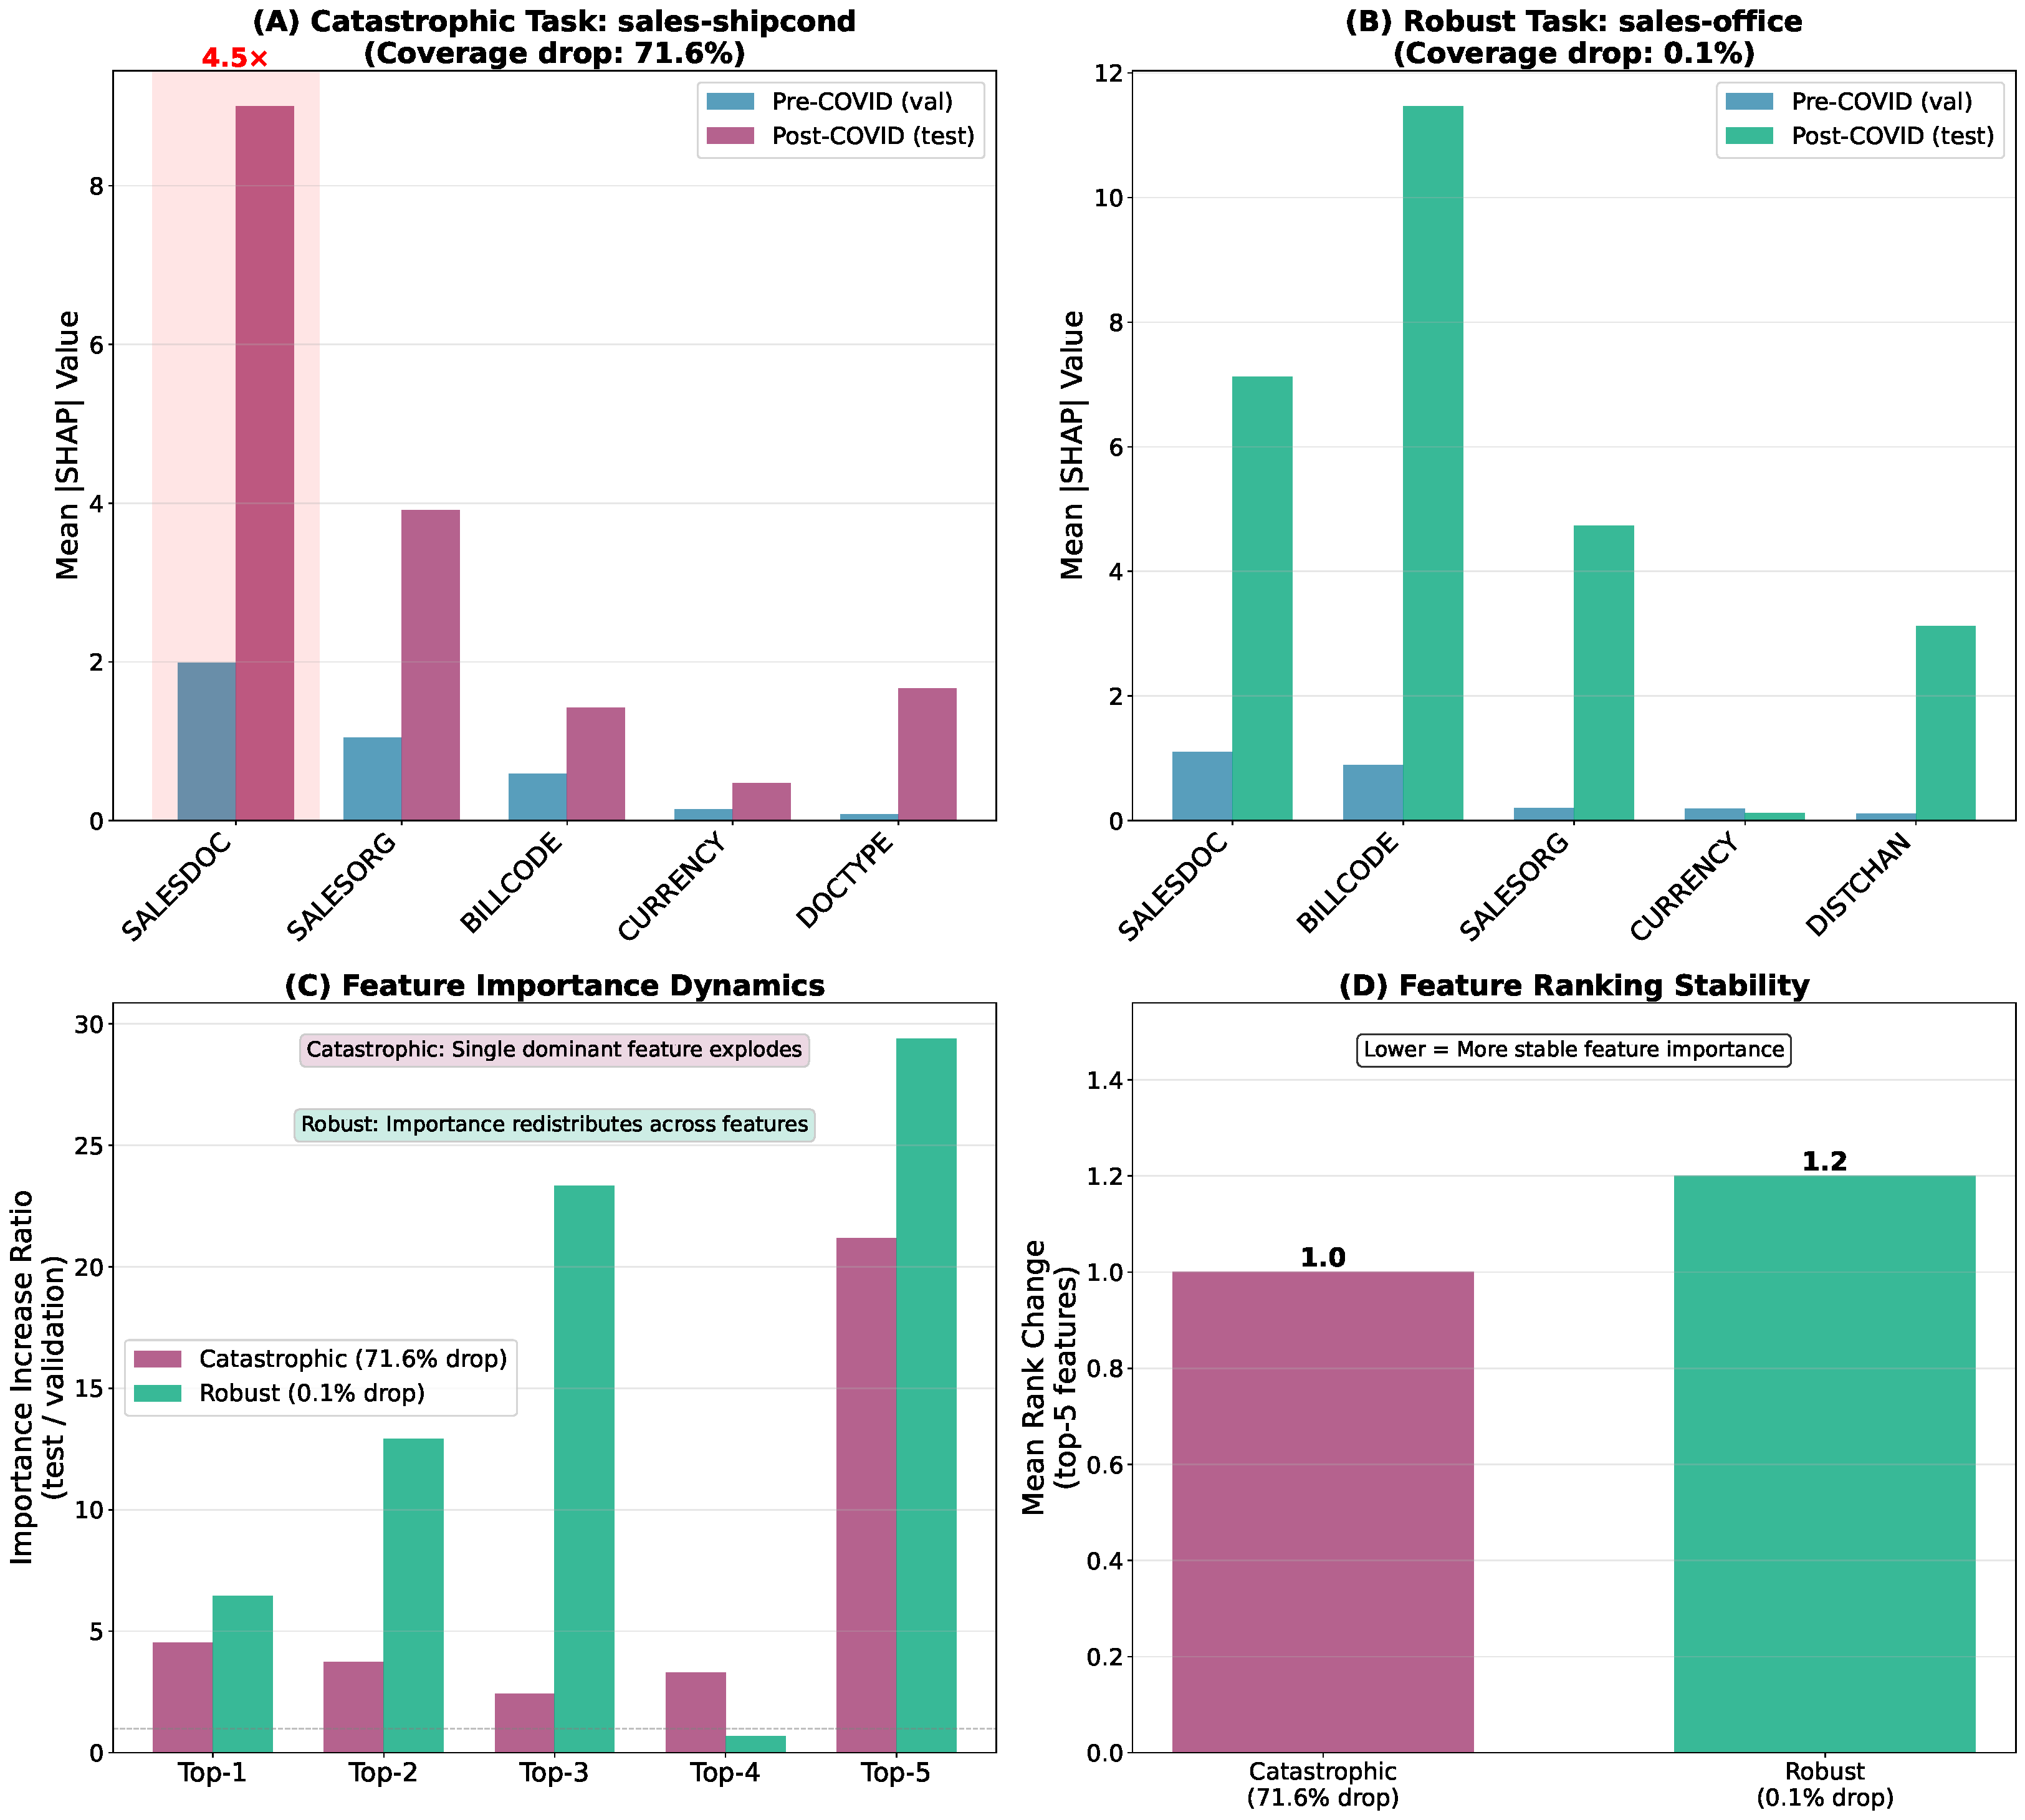
\includegraphics[width=0.94\linewidth]{../figures/figure3_feature_importance.pdf}}
\end{center}
{\fontsize{18}{22}\selectfont\itshape Fig 2: Mechanism. A/B compare SHAP mass before vs. after COVID shift; C/D show whether the failure is driven by one feature or distributed dependence.\par}
\vspace{0.12em}
{\fontsize{17}{21}\selectfont
\setlength{\tabcolsep}{0.25em}
\begin{tabular}{@{}>{\raggedright\arraybackslash}p{0.49\linewidth}>{\raggedright\arraybackslash}p{0.49\linewidth}@{}}
\textbf{A. Failure:} post-COVID SHAP mass jumps onto one feature. &
\textbf{B. Robust:} importance remains spread across features. \\
\textbf{C. Ratio:} failing task has a top-feature spike. &
\textbf{D. Stability:} robust dependence changes less; the top features keep similar order after shift. \\
\end{tabular}\par
}
\vspace{0.2em}
\begin{center}
\fcolorbox{alertred}{red!7}{\parbox{0.93\linewidth}{\centering
\vspace{0.16em}
{\fontsize{21}{26}\selectfont\bfseries\color{alertred}Takeaway: high-$C$ GBMs create a single point of failure.}\\[-0.02em]
{\fontsize{17}{21}\selectfont When the dominant feature shifts, APS scores rise and CP coverage drops.}
\vspace{0.16em}
}}
\end{center}
}

\end{minipage}%
\hfill
\begin{minipage}[t]{0.29\textwidth}
\vspace{0pt}

\posterbox{External Specificity}{%
\vspace{0.65cm}
\fontsize{22}{27}\selectfont
\textbf{4 robust external checks, all $C<40\pct$}\par
{\fontsize{16}{20}\selectfont\textit{Distinct from the $n=16$ UCI endpoint; tests specificity: low $C$ should predict robust coverage.}}
\begin{center}
\renewcommand{\arraystretch}{1.12}
{\fontsize{18}{22}\selectfont
\begin{tabular}{lccc}
\toprule
\textbf{Dataset} & \textbf{C} & \textbf{Drop} & \textbf{Pred.} \\
\midrule
CivilComments & 26.2\pct & -0.7pp & Robust \\
Amazon & 1.9\pct & +0.4pp & Robust \\
Covertype & 12.5\pct & +8.0pp & Robust \\
Adult & 27.5\pct & +1.4pp & Robust \\
\bottomrule
\end{tabular}}
\end{center}
\begin{center}
\fcolorbox{successgreen}{green!8}{\parbox{0.82\linewidth}{\centering
\vspace{0.18em}
{\fontsize{42}{50}\selectfont\bfseries\color{successgreen}91.7\pct}\\[-0.03em]
{\fontsize{20}{25}\selectfont 11/12 tasks correctly flagged}\\[-0.02em]
{\fontsize{15}{18}\selectfont task-level robust/at-risk threshold rule}
\vspace{0.18em}
}}
\end{center}
}

\vspace{0.75cm}

\posterbox{Next Steps}{%
\vspace{0.65cm}
\fontsize{22}{27}\selectfont
\textbf{Future directions}
\begin{itemize}
    \item Gradient-based explanations for neural networks
    \item Automatic mitigation to reduce concentration
    \item Tighter distribution-specific coverage bounds
\end{itemize}
\vspace{0.2em}
\textbf{Open questions}
\begin{itemize}
    \item Can models be intrinsically \textbf{low-concentration}?
    \item Does the cutoff hold prospectively across domains?
    \item Can streaming CP trigger mitigation before failure?
\end{itemize}
}

\end{minipage}

\vspace{0.85cm}

\begin{center}
\begin{tikzpicture}
\node[draw=uaiblue, line width=2.2pt, fill=uaiblue!4, rounded corners=8pt, inner sep=18pt, text width=0.965\textwidth, align=left, drop shadow={shadow xshift=1.4pt, shadow yshift=-1.4pt, opacity=0.10}] (box) {%
\begin{minipage}[t]{0.34\linewidth}
\raggedright
\fcolorbox{uaiorange}{white}{\parbox{0.95\linewidth}{%
\begin{minipage}{0.58\linewidth}
{\fontsize{26}{32}\selectfont\bfseries\color{uaiblue}Paper \& Code}\par\vspace{0.25em}
{\fontsize{18}{22}\selectfont\texttt{github.com/ChorokLeeDev/}}\par
{\fontsize{18}{22}\selectfont\texttt{conformal-covid-uai2026}}\par\vspace{0.45em}
{\fontsize{24}{30}\selectfont\bfseries\color{uaiblue}Contact}\par\vspace{0.2em}
{\fontsize{18}{22}\selectfont\texttt{chorok.lee@kaist.ac.kr}}
\end{minipage}
\hfill
\begin{minipage}{0.33\linewidth}
\centering
\fcolorbox{uaiblue}{white}{
\includegraphics[width=5.2cm]{qr_code.png}}\par\vspace{0.15em}
{\fontsize{15}{18}\selectfont\bfseries Scan for paper \& code}
\end{minipage}
}}
\end{minipage}
\hfill
\begin{minipage}[t]{0.30\linewidth}
\raggedright
{\fontsize{25}{30}\selectfont\bfseries\color{uaiblue}Why Not Standard Shift Tests?}\par\vspace{0.35em}
{\fontsize{20}{25}\selectfont MMD, C2ST, and PSI detect shift across SALT tasks, but correlate weakly with coverage drop: \textbf{$\rho \leq 0.19$}. They say ``shift happened,'' not which CP model fails.}
\end{minipage}
\hfill
\begin{minipage}[t]{0.30\linewidth}
\raggedright
{\fontsize{25}{30}\selectfont\bfseries\color{uaiblue}Scope \& Limits}\par\vspace{0.35em}
{\fontsize{20}{25}\selectfont Best supported for \textbf{GBM multiclass classifiers}. Treat \textbf{35--45\pct} as uncertain; RF and MLP may show different failure modes.}
\end{minipage}
};
\node[fill=uaiblue, text=white, font=\bfseries\LARGE, rounded corners=4pt, inner sep=9pt, anchor=south west] at ($(box.north west)+(0.45cm,-0.22cm)$) {Paper, Code \& Context};
\end{tikzpicture}
\end{center}

\end{document}
